\documentclass[border=2pt]{standalone}
\usepackage{pgfplots}
\pgfplotsset{compat=1.18}
\begin{document}
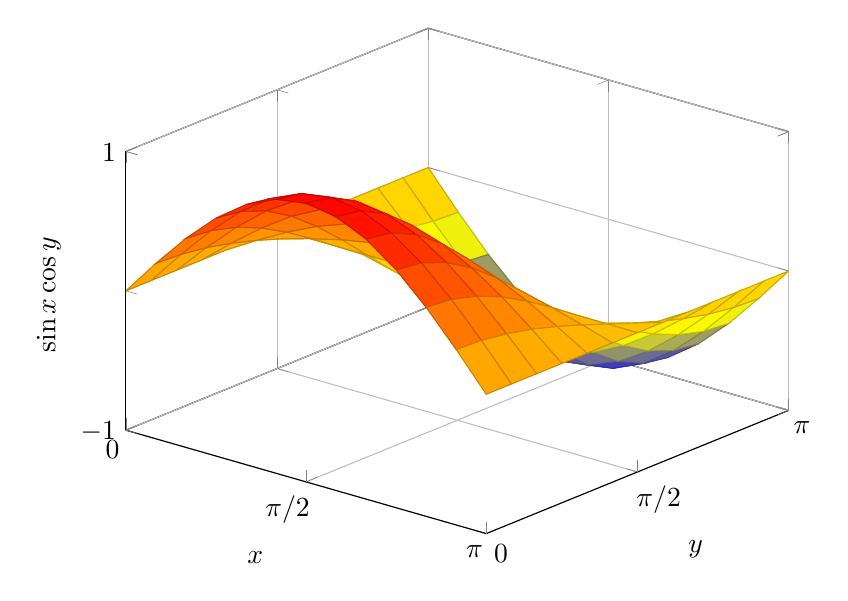
\begin{tikzpicture}
  \begin{axis}[
    width=10cm,
    height=8cm,
    view={40}{30},
    domain=0:3.14159,
    y domain=0:3.14159,
    samples=13,
    xmin=0,
    xmax=3.14159,
    ymin=0,
    ymax=3.14159,
    zmin=-1,
    zmax=1,
    xtick={0,1.5708,3.14159},
    xticklabels={$0$,{$\pi/2$},{$\pi$}},
    ytick={0,1.5708,3.14159},
    yticklabels={$0$,{$\pi/2$},{$\pi$}},
    ztick={-1,0,1},
    zticklabels={$-1$,,$1$},
    grid=major,
    xlabel={$x$},
    ylabel={$y$},
    zlabel={$\sin x\cos y$}
  ]
    \addplot3[surf] {sin(deg(x))*cos(deg(y))};
  \end{axis}
\end{tikzpicture}
\end{document}
